
\documentclass[MAIN.tex]{subfiles} 
\begin{document} 
	\begin{frame}
		\frametitle{Probability Distributions}
	A probability distribution is a table or an equation that links each outcome (or range of outcomes) 
	of a statistical experiment with its probability of occurrence.\\
	\bigskip
	\textbf{Two Families}
	\begin{itemize}
	\item Discrete Distributions (i.e. Count Variables  - Integers )
	\item Continuous Distributions (i.e. Continuous Variables - Real Numbers )
	\end{itemize}
	
	\end{frame}
%================================================================================== %
\begin{frame}
	\frametitle{Discrete distributions}
\begin{itemize}
\item Benford Distribution
\item Bernouilli distribution
\item Binomial distribution
\item Hypergeometric distribution
\item Geometric distribution
\item Multinomial distribution
\item Negative binomial distribution
\item Poisson distribution
\item Zipf's law
\end{itemize}
\end{frame}

%================================================================================== %
\begin{frame}
\frametitle{Continuous distributions}
\begin{itemize}
\item Beta and Dirichlet distributions
\item Cauchy distribution
\item Chi Square distribution
\item Exponential distribution
\item Fisher-Snedecor distribution
\item Gamma distribution
\item Levy distribution
\item Log-normal distribution
\item Normal and related distributions
\item Pareto Distributions
\item Student's t distribution
\item Uniform distribution
\item Weibull distribution
\item Extreme values and related distribution
\item Distribution in circular statistics
\end{itemize}
\end{frame}
%================================================================================== %
\begin{frame}
	\begin{figure}
		\centering
		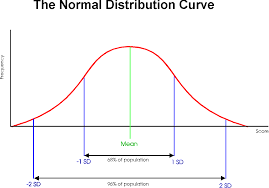
\includegraphics[width=0.9\linewidth]{images/bellcurve}
	\end{figure}

\end{frame}
%================================================================================== %
\begin{frame}
\frametitle{The Normal Distribution}
\textbf{Normal Probability Distribution}
\large
\begin{itemize}
\item Cornerstone of every undergraduate statistics module.
\item Basis of a substantial body of statistical theory
\item Central Limit Theorem - basis of Statistical Inference (i.e. Hypothesis Tesing, Confidence Intervals).

\end{itemize}
\end{frame}
%================================================================================== %

\begin{frame}
	\begin{figure}
\centering
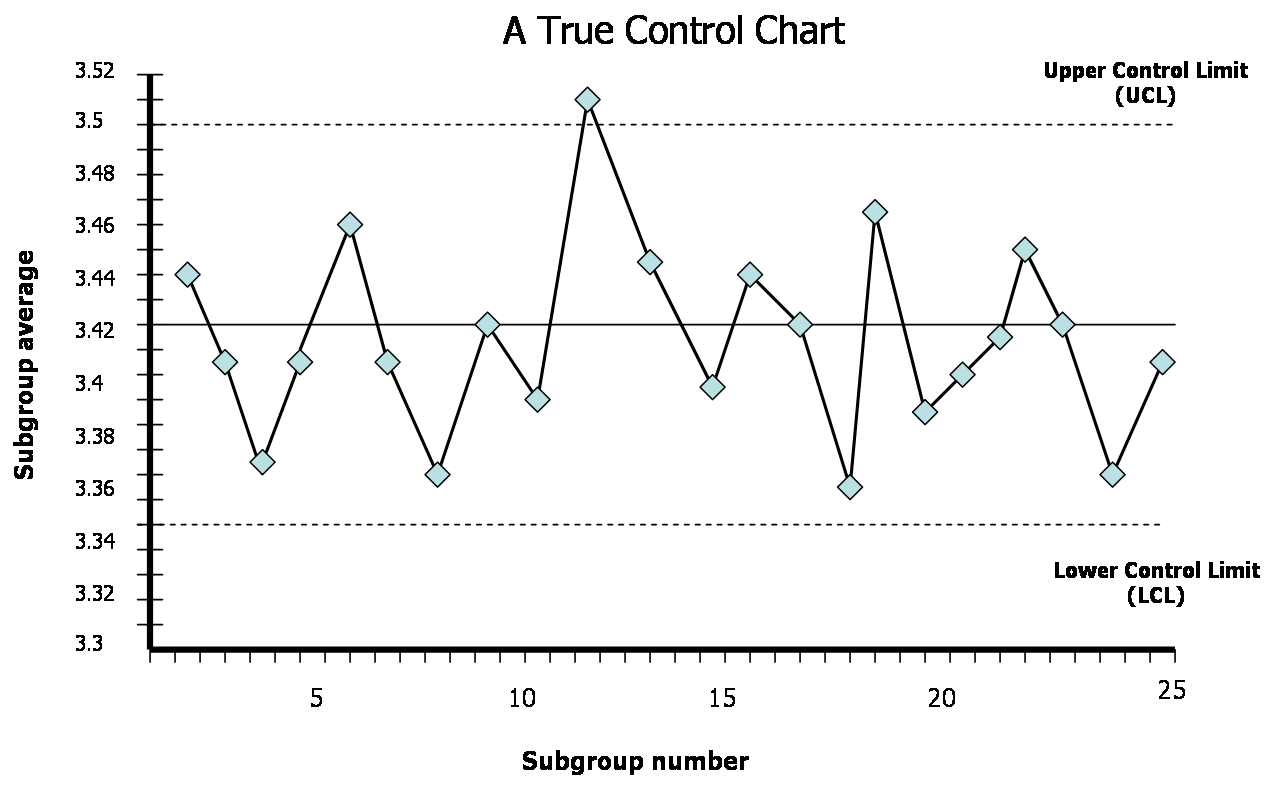
\includegraphics[width=1.1\linewidth]{images/controlchart}
\end{figure}
\end{frame}
%================================================================================== %

\begin{frame}
	
\begin{figure}
\centering
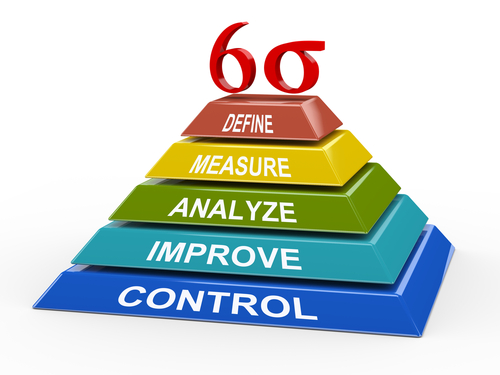
\includegraphics[width=0.99\linewidth]{images/sixsigmalogo}

\end{figure}

\end{frame}
%================================================================================== %

\begin{frame}
	\begin{figure}
\centering
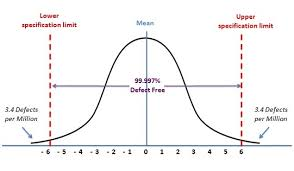
\includegraphics[width=1.05\linewidth]{images/sixsigma}
\end{figure}

	
	
\end{frame}
%================================================================================== %

\begin{frame}

\begin{figure}
\centering

\includegraphics[width=0.7\linewidth]{images/sixsigmabook}

\end{figure}

\end{frame}

%================================================================================== %
\begin{frame}
\frametitle{Compendium of Probability Distributions}
\begin{figure}
\centering

\includegraphics[width=1.05\linewidth]{images/vosecompendium}
\end{figure}
\end{frame}
%================================================================================== %
\begin{frame}
	\frametitle{Compendium of Probability Distributions}
		\begin{figure}
\centering
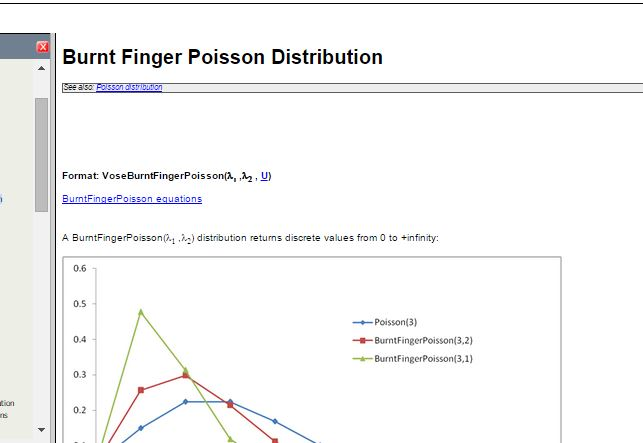
\includegraphics[width=0.9\linewidth]{images/burntfinger}

\end{figure}

\end{frame}
%================================================================================ %
\begin{frame}
	\frametitle{Compendium of Probability Distributions}
\textbf{Burnt Finger Poisson Disribution}
\begin{itemize}
\item This type of situation occurs when, for example, an individual has an expected rate of accidents $\lambda_1$, but if an accident occurs the individual will become more careful (his/her ``fingers got burned") so that for the rest of the modeled time a new, lower expected accident rate $\lambda_1$ applies.
\end{itemize}
\end{frame}
%================================================================================ %
\begin{frame}
	\frametitle{Compendium of Probability Distributions}
	\textbf{Burr Disribution}
\begin{itemize}
\item The Burr distribution is a right-skewed distribution bounded at the minimum value of a. b is a scale parameter while c and d control its shape. 

\item It is frequently used to model insurance claim sizes, and is sometimes considered as an alternative to a Normal distribution when data show slight positive skewness.
\end{itemize}
\end{frame}
%================================================================================ %
\begin{frame}
	\frametitle{Compendium of Probability Distributions}
	\textbf{Burr Disribution}

Burr(0,1,c,d) is a unit Burr distribution. 
Examples of the Burr distribution are given below:

\begin{figure}
\centering
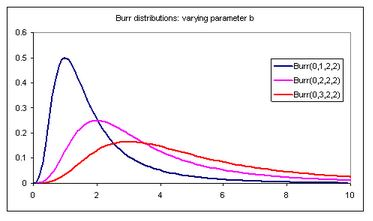
\includegraphics[width=0.7\linewidth]{images/burrdistribution}
\caption{}
\label{fig:burrdistribution}
\end{figure}


\end{frame}
%================================================================================================================ %
\begin{frame}
\frametitle{Skellam distribution}
\large
\begin{itemize}

\item The \textbf{Skellam distribution} is the discrete probability distribution of the difference $n_1-n_2$ of two statistically independent random variables $N_1$ and $N_2$ each having Poisson distributions with different expected values $\mu_1$ and $\mu_2$.
\item It is useful in describing the statistics of the difference of two images with simple photon noise.
\item It is also useful in describing the \textbf{point spread distribution} in sports where all scored points are equal, such as baseball, hockey and soccer.
\end{itemize}
\end{frame}

\begin{frame}
\frametitle{Skellam distribution}
\large
Package no longer on CRAN - seemingly implemented on some other pacakges though.
	\begin{figure}
\centering

\includegraphics[width=0.7\linewidth]{images/skellampackage}
\caption{}
\label{fig:skellampackage}
\end{figure}
\end{frame}

\begin{frame}
	\begin{figure}
\centering
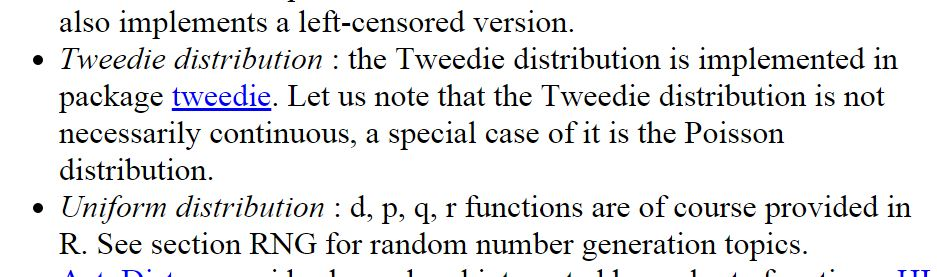
\includegraphics[width=1.05\linewidth]{images/TweedieCRAN}
\caption{}
\label{fig:TweedieCRAN}
\end{figure}

\end{frame}

\begin{frame}
	\begin{figure}
\centering
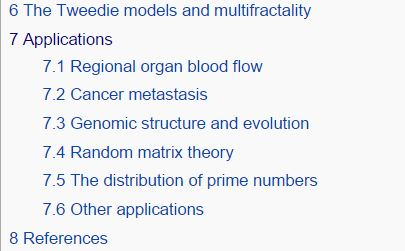
\includegraphics[width=0.9\linewidth]{images/tweedie}
\caption{}
\label{fig:tweedie}
\end{figure}

\end{frame}
%================================================================================ %
\begin{frame}
	\begin{figure}
		\centering
		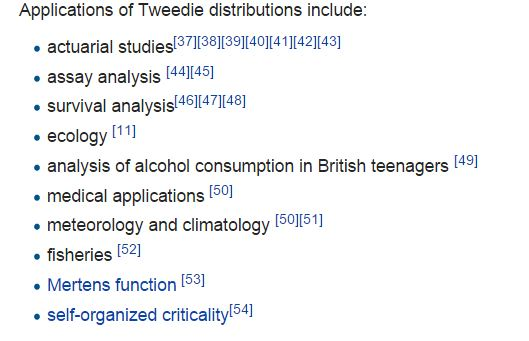
\includegraphics[width=1.05\linewidth]{images/tweedie2}

	\end{figure}
	
\end{frame}
\begin{frame}
	\begin{figure}
\centering
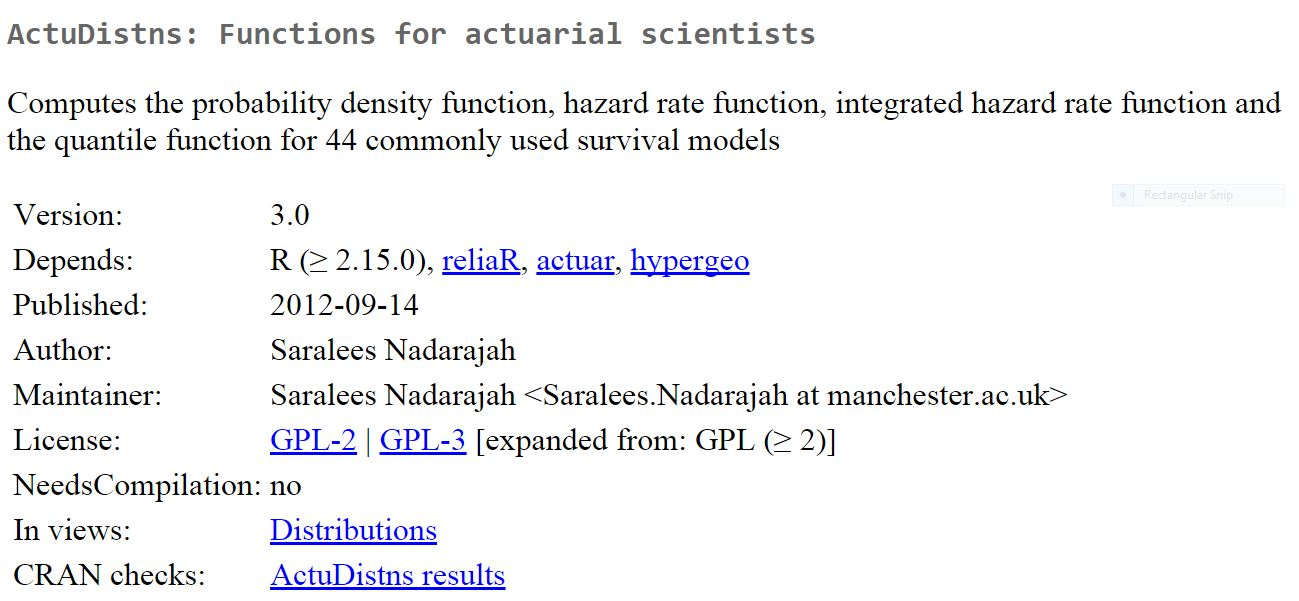
\includegraphics[width=1.05\linewidth]{images/ActuDistns}

\end{figure}

\end{frame}
%================================================================================ %
\begin{frame}
	\frametitle{Compendium of Probability Distributions}
	\textbf{Braford Distribution}
\large
\begin{framed}
	\begin{quote}
	The theory has a lot of implications in researching and investment in periodicals: for example, how many journals an institute should subscribe to, or one should review in a study. It also gives a guide for advertising, by identifying the first third of journals that have the highest impact, helps determine whether journals on a new(ish) topic (or arena like e-journals) have reached a stabilised population, and test the efficiency of Web browsers.
\end{quote}
\end{framed}
\end{frame}

%================================================================================= %
\begin{frame}
	\frametitle{Main Functions for \texttt{R}}
\begin{description}
\item[\texttt{d}] - probability density function
\item[\texttt{p}] - cumulative distribution function
\item[\texttt{q}] - quantile function
\item[\texttt{r}] - random number generation function
\end{description}

\end{frame}

\begin{frame}
\frametitle{Some Probability Distributions in \texttt{R}}
	\begin{figure}
\centering
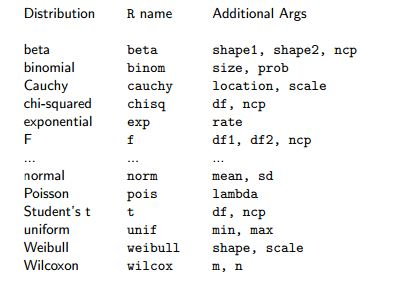
\includegraphics[width=0.9\linewidth]{images/stems}
\end{figure}
\end{frame}
%=========================================================================================================== %

\begin{frame}
\begin{figure}
\centering
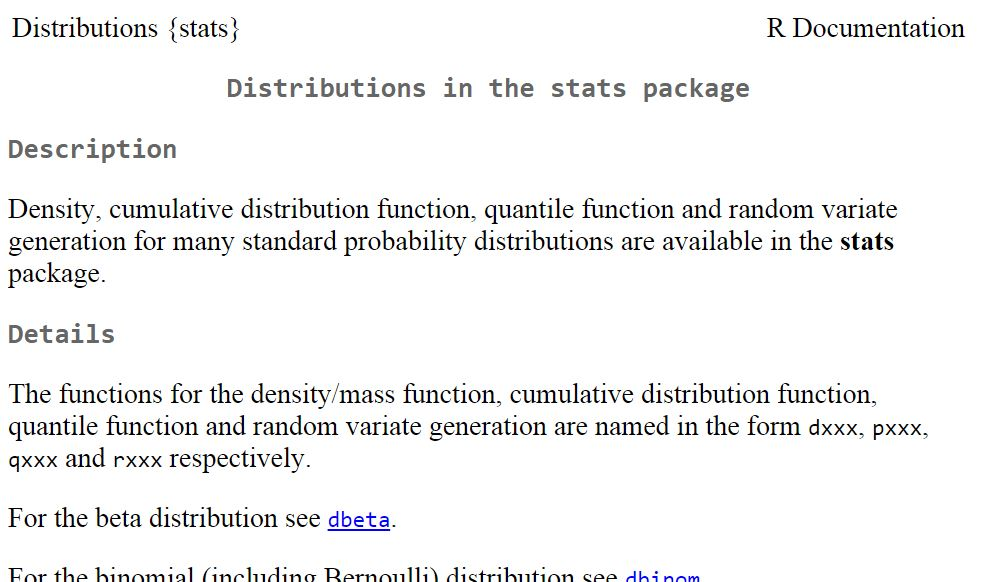
\includegraphics[width=1.05\linewidth]{images/helpdistributions}
\end{figure}
\end{frame}
%=========================================================================================================== %
\begin{frame}
	\frametitle{The Birthday Problem}
\begin{itemize}
\item How many people have to be in a room for there to be a better than 50/50 chance of two people sharing a birthday?
\end{itemize}	
	\begin{figure}
\centering
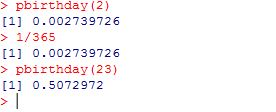
\includegraphics[width=0.7\linewidth]{images/pbirthday}
\end{figure}

\end{frame}
%================================================================================= %
\begin{frame}
	\begin{figure}
		\centering
		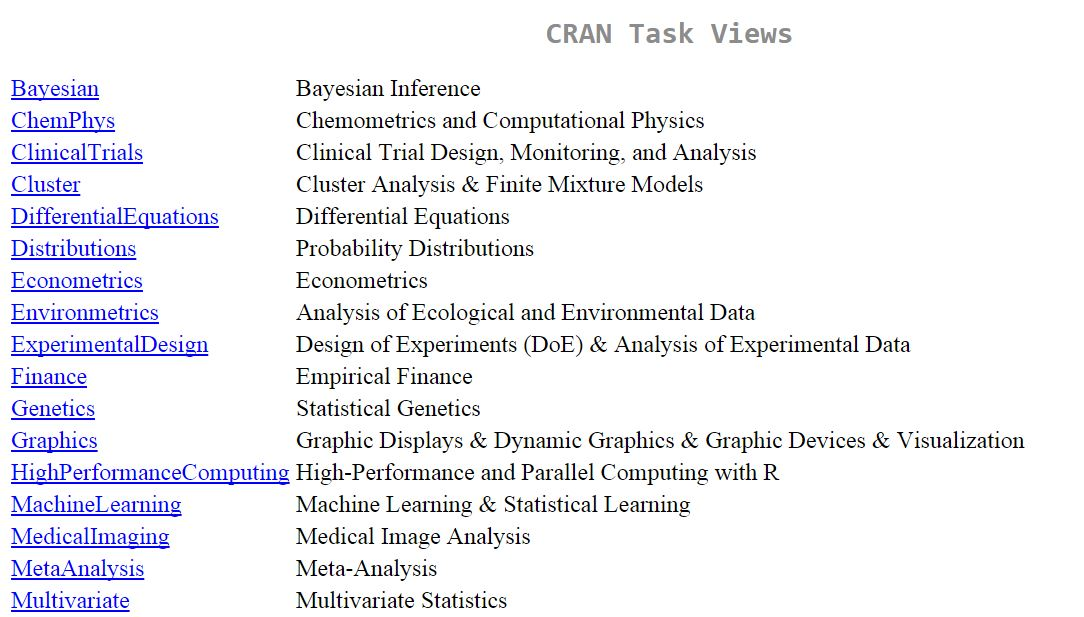
\includegraphics[width=1.05\linewidth]{images/CRANTaskviewALL}
		
	\end{figure}
\end{frame}
%================================================================================= %
\begin{frame}
	\begin{figure}
\centering
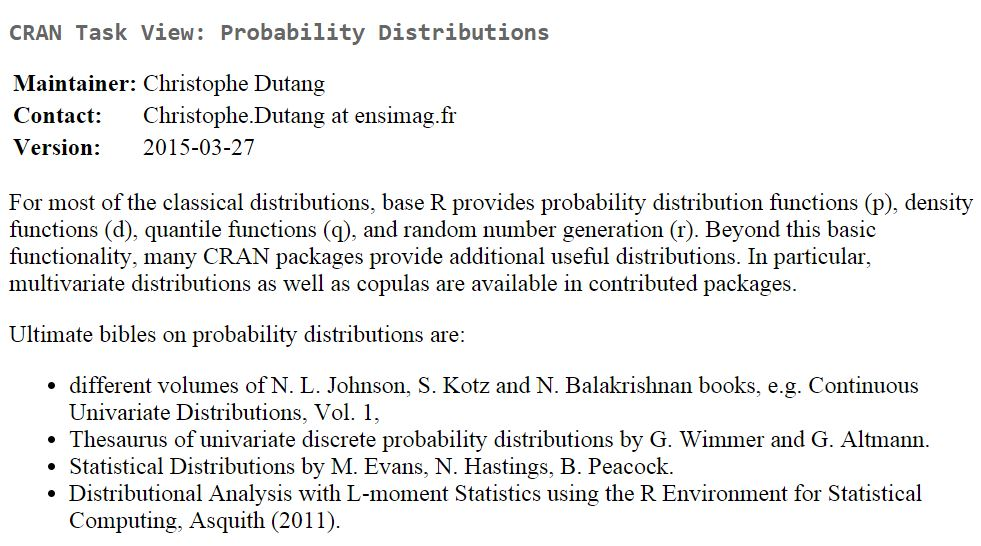
\includegraphics[width=1.05\linewidth]{images/CRANTaskview}

\end{figure}
\end{frame}
%================================================================================= %
\begin{frame}

	\begin{figure}
\centering
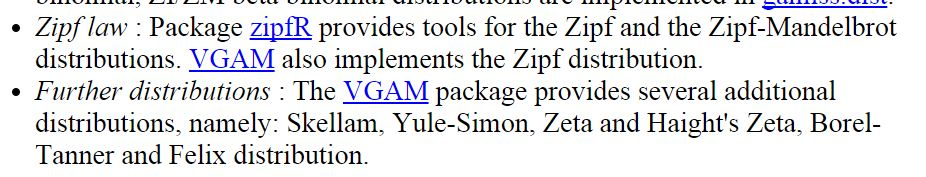
\includegraphics[width=0.7\linewidth]{images/CRANzipf}

\end{figure}

\end{frame}
%================================================================================== %
\begin{frame}
\frametitle{The VGAM package}
	\begin{figure}
\centering
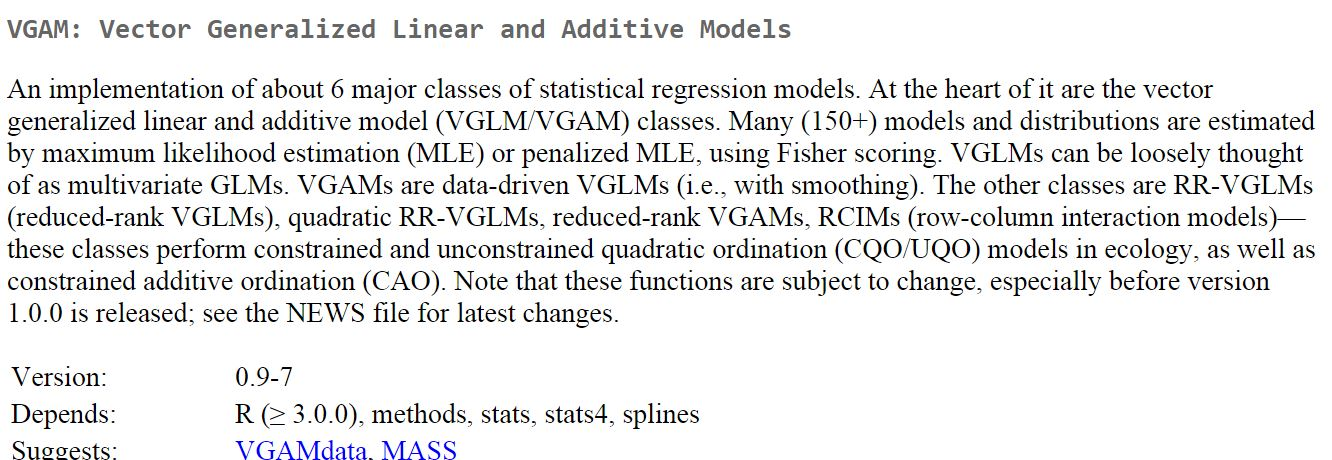
\includegraphics[width=1.05\linewidth]{images/VGAM}

\end{figure}

\end{frame}
%==================================================================================== %
\begin{frame}
	\begin{figure}
\centering
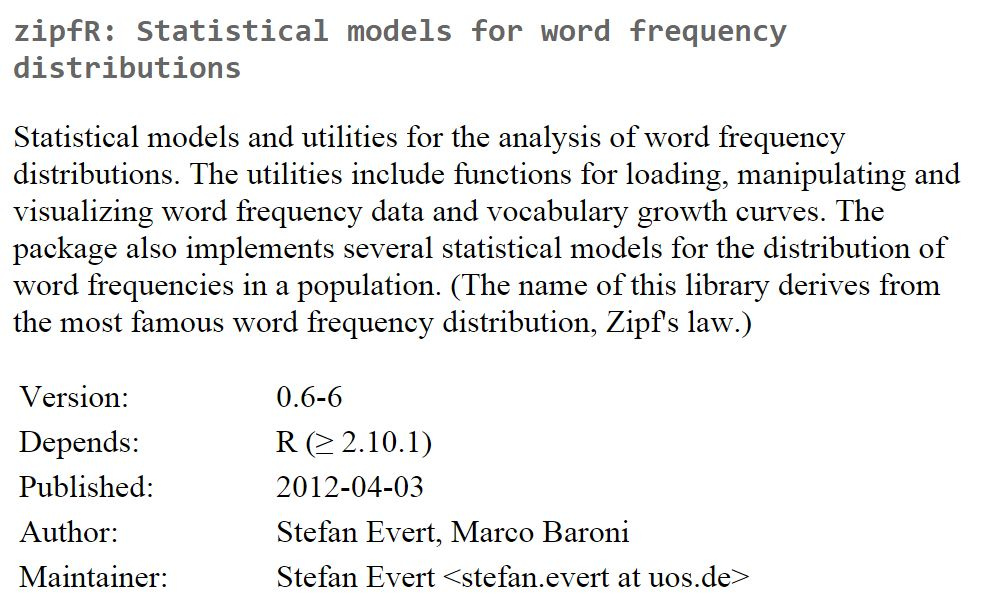
\includegraphics[width=1.05\linewidth]{images/zipfR}

\end{figure}

\end{frame}
%================================================================================= %
\begin{frame}
	
\begin{figure}
\centering
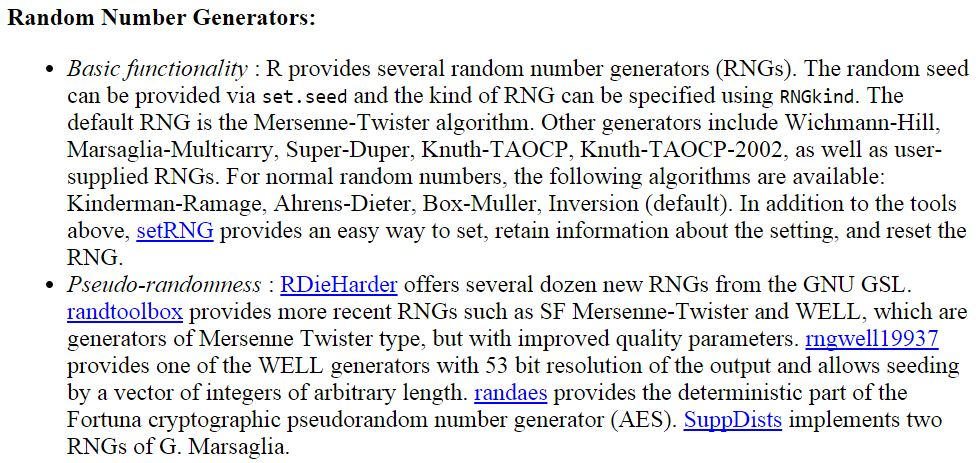
\includegraphics[width=1.05\linewidth]{images/CRANrng}
\end{figure}

\end{frame}
%================================================================================= %
\begin{frame}
	\begin{figure}
\centering
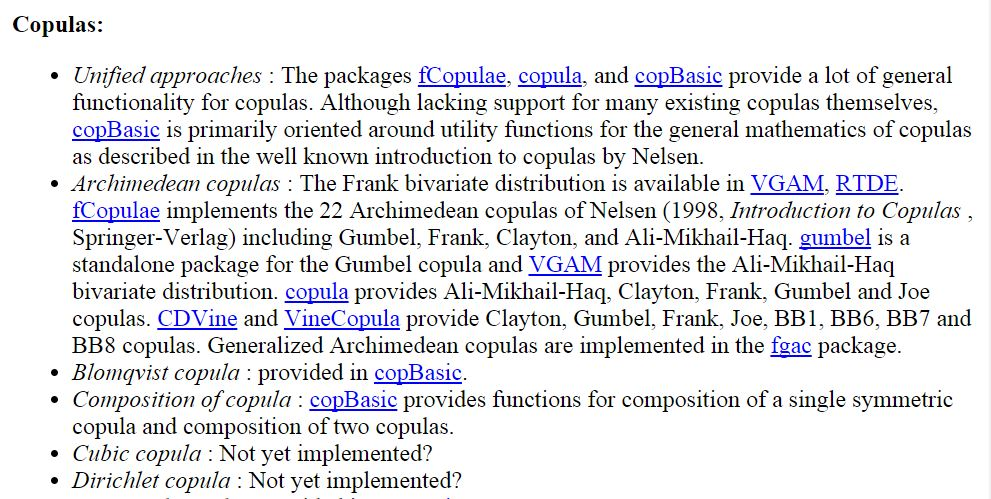
\includegraphics[width=1.05\linewidth]{images/CRANcopulas}

\end{figure}

\end{frame}
%================================================================================= %
\end{document}
